\documentclass{article}
\usepackage[utf8]{inputenc}
\usepackage{graphicx}
\usepackage[italian]{babel} % lingua italiana
\usepackage{hyperref}
\usepackage{geometry}
\usepackage{svg}

\graphicspath{ {./images/} }

\title{Sistema di una Biblioteca Digitale}
\author{Gennaro Nappo - Giovanni Riccio\\N86004294 - N86004316}
\date{Anno accademico 2022-2023}

\begin{document}

\maketitle

\includegraphics[width = 141mm]{images/Logo.jpg}

\newpage
\tableofcontents

\newpage
\section{Progettazione concettuale}

\subsection{Analisi dei requisiti}
In questa sezione sono individuate le informazioni rilevanti per poter soddisfare le richieste informative e funzionali del DB, in particolare sono individuate le \textit{Entità}, le \textit{Relazioni}, i \textit{Vincoli} e le operazioni che gli utenti possono effettuare più frequentemente.

\begin{quote}
\textit{"Si sviluppi un sistema informativo, composto da una base di dati relazionale per la gestione di una biblioteca digitale"}
\end{quote}

Come da richiesta, consideriamo di gestire un'unica grande biblioteca digitale, cioè un catalogo di elementi che gli utenti possono consultare, quindi non necessiteremo di un'entità \textit{Biblioteca} per poter rappresentare la biblioteca del mondo reale.

\begin{quote}
\textit{"Gli elementi che possono essere inclusi nella biblioteca digitale sono di due tipi: articoli scientifici e libri (didattici o romanzi). Per ognuno di essi, devono essere specificati il titolo, l’anno di pubblicazione, gli autori, l’editore e definire le modalità di fruizione (cartaceo, digitale o audiolibro)."}
\end{quote}

Abbiamo la necessità di dover rappresentare come entità gli elementi inclusi nella biblioteca, cioè gli articoli scientifici e i libri, quindi avremo le entità \textit{articolo\_scientifico} e \textit{libro}.\\
Alcuni articoli scientifici saranno introdotti in dei fascicoli, che a loro volta faranno parte di riviste, quindi avremo bisogno delle entità \textit{rivista} e \textit{fascicolo}, quest'ultima sarà un'entità debole in quanto un'istanza di tale entità per essere identificata univocamente necessita della chiave primaria dell'entità \textit{rivista}, ovvero l'attributo ISSN.\\
Ogni libreria sarà gestita da un utente che possiede una partita IVA, quindi avremo bisogno di un'entità \textit{venditore}, ovvero una specializzazione dell'entità \textit{utente}, che avrà un attributo PartitaIVA e quindi potrà gestire una libreria. Le librerie saranno rappresentate dall'entità \textit{libreria} e gli elementi che possiedono, sono rappresentati dalle seguenti sottoclassi dell'entità \textit{elemento}: \begin{itemize} 
\item \textit{fascicoli}; 
\item \textit{serie};
\item \textit{libri}.
\end{itemize}
Ognuno di queste entità avrà il titolo, la data di pubblicazione, gli autori e l'editore come attributi.\\
In oltre la modalità di fruizione sarà definita come attributo della relazioe \textit{possesso}, che mette in relazione le entità \textit{libreria} ed \textit{elemento}, questa relazione avrà anche un attributo Quantita per avere traccia della quantità di elementi disponibili di ogni libreria.

\begin{quote}
\textit{"Per i libri è importante definire una eventuale presentazione. Un libro può anche far parte di una collana, la quale può raggruppare tutti libri che condividono una determinata caratteristica."}
\end{quote}

Si richiede di gestire eventuali presentazioni dei libri, ed eventuali collane alle quali apparterranno dei libri, quindi necessiteremo delle entità \textit{collana} e \textit{presentazione}.

\begin{quote}
\textit{Per le pubblicazioni, andare a definire in quale rivista (nome, argomento, anno di pubblicazione, responsabile della rivista) o in quale conferenza (luogo della conferenza, data di inizio e data fine conferenza, struttura organizzatrice) è stato pubblicato.}
\end{quote}

 Per gli articoli scientifici è importante avere traccia in quale rivista sono introdotti, ovvero in quale rivista è contenuto il fascicolo in cui è stato pubblicato l'articolo, e in quale conferenza sono stati esposti, quindi avremo bisogno dell'entità \textit{rivista} che avrà i seguenti attributi: Titolo; Argomento; Anno di pubblicazione e Responsabile, quest'entità sarà in relazione con l'entità \textit{fascicolo}, che a sua volta sarà in relazione con l'entità \textit{articolo\_scientifico}. In oltre necessiteremo anche dell'entità \textit{conferenza} con i seguenti attributi: Luogo, che sarà formato dall'indirizzo e dalla struttura organizzatrice; Data di Inizio e Data di Fine. Questa entità sarà in relazione con l'entità \textit{articolo\_scientifico}. 

\begin{quote}
\textit{per ogni libro, è necessario specificare dove può essere acquistato. Un romanzo può avere anche uno o più seguiti. In tal caso, è importante prevedere un’interrogazione che permette di recuperare tutte le librerie dai quali è possibile acquistare l’intera serie dei libri. Non appena una serie sarà disponibile per l’acquisto da almeno una libreria, il sistema notificherà la disponibilità all’utente.}
\end{quote}

Per permettere al sistema di specificare dove può essere acquistato ogni elemento posseduto da una libreria (fascicolo di una rivista, libro e serie di libri) avremo bisogno della relazione \textit{possesso} tra le entità \textit{libreria} ed \textit{elemento}.
Una serie sarà formata da un certo numero di libri e sarà rappresentata dall'entità \textit{serie}, che sarà in relazione con l'entità \textit{libro} tramite l'associazione \textit{inserimento}.
Per inviare la notifica a gli utenti interessati ad una serie disponibile, utilizzeremo:
\begin{itemize}
    \item Una relazione \textit{recensione} tra \textit{utente} ed \textit{elemento}: questa relazione permetterà di avere traccia di una valutazione e una recensione (presenti rispettivamente negli attributi Valutazione e Testo) fatte dall'utente. In oltre avrà un attributo Preferito che indica gli utenti che hanno tra i preferiti degli elementi, e quindi indicherà anche se l'utente, che partecipa a questa relazione, vuole ricevere una notifica quando la serie associata è completamente disponibile in qualche libreria;
    \item Una relazione \textit{notifica} tra le entità \textit{utente} e \textit{serie}: che conterrà tutte le notifiche inviate agli utenti che partecipano alla relazione \textit{recensione} e che hanno l'attributo Preferito a 'true' (e quindi hanno attivato le notifiche per una certa serie), ogni volta che una serie associata a tali utenti è disponibile presso qualche libreria.
    \item Trigger e Funzioni che si occuperanno di inviare automaticamente le notifiche quando:
    \begin{itemize}
        \item Un'utente attiva le notifiche per una serie già disponibile, cioè nella relazione \textit{recensione} avviene un inserimento o una modifica in cui l'attributo Preferito assume il valore 'true' e l'elemento associato a tale utente è una serie;
        \item Una libreria inizia a possedere una serie per la quale un utente ha attivato le notifiche, cioè nella relazione \textit{possesso} avviene un inserimento o una modifica in cui l'attributo Quantità ha un valore maggiore di 0 oppure la modalita di fruizione è 'Digitale' o 'AudioLibro' (quindi non è necessario specificare la quantità disponibile).
    \end{itemize} 
\end{itemize}

\newpage
\subsection{Schema concettuale}
\begin{figure}[htp!]
    \includegraphics[width=0.75\columnwidth]{images/DiagrammaER v1.4.1(girato).png}
\end{figure}

\newpage
\section{Ristrutturazione del modello concettuale}
Prima di poter passare allo schema logico è necessario ristrutturare il diagramma delle classi.

\subsection{Analisi delle ridondanze}
L'editore di una rivista può essere ricavato consultando l'attributo 'Editore' dell'entità \textit{fascicolo}, quindi non è necessario inserire tale attributo nell'entità \textit{rivista}. L'attributo 'Ordine' della relazione \textit{Inserimento} può essere calcolato contando il numero di libri associati a una serie, quindi anche questo attributo non verrà inserito nella sua relazione.\\ In questo modo avremo una minore occupazione di spazio e degli aggiornamenti meno pesanti.

\subsection{Analisi delle generalizzazioni}
Per rimuovere la generalizzazione totale overlapping "utente", accorpiamo le entità figlie \textit{venditore} e \textit{standard} nell'entità padre \textit{utente}.
Per quanto riguarda la generalizzazione disgiunta totale "elemento" procediamo accorpando l'entià padre \textit{elemento} nelle entità figlie \textit{fascicolo}, \textit{libro} e \textit{serie}.

\subsection{Eliminazione degli attributi multivalore}
Nelle entità \textit{articolo\_scientifico} e \textit{libro} abbiamo un attributo multivalore (e strutturato) \textit{Autore} che ci permette di rappresentare gli autori che hanno scritto un libro e/o un articolo scientifico, quindi abbiamo creato delle apposite entità esterne.

\subsection{Eliminazione degli attributi strutturati}
L'entità \textit{conferenza} contiene l'attributo composto \textit{Luogo} che è formato da \textit{Struttura Organizzatrice} e \textit{Luogo Conferenza}, quest'ultimo a sua volta è composto da \textit{Nazione}, \textit{Città} e \textit{Indirizzo}. Quindi trascuriamo la struttura dell'attributo \textit{Luogo Conferenza} rendendolo un unico attributo, poi estraiamo gli attributi \textit{Luogo Conferenza} e \textit{Struttura Organizzatrice} inserendo nell'entità \textit{conferenza} i corrispondenti attributi \textit{Luogo} e \textit{Struttura organizzatrice}.\\
L'attributo composto \textit{Luogo} dell'entità \textit{presentazione} è formato da: \textit{Luogo Presentazione} che a sua volta contiene \textit{Nazione}, \textit{Città} e \textit{Indirizzo}; e \textit{Struttura Organizzatrice}, che a sua volta contiene \textit{Sala} e \textit{Nome}. Trascuriamo la struttura dell'attributo \textit{Struttura Organizzatrice} rendendolo un unico attributo, e facciamo la stessa operazione con l'attributo  \textit{Luogo Presentazione}, poi  estraiamo gli attributi  \textit{Luogo Presentazione} e \textit{Struttura Organizzatrice} inserendo nell'entità \textit{presentazione} i corrispondenti attributi \textit{Luogo} e \textit{Struttura}.\\
Un'altro attributo composto è \textit{Responsabile} nell'entità \textit{rivista}, composto dagli attributi \textit{Nome} e \textit{Cognome}. Anche in questo caso procediamo estraendo questi attributi e introduciamo nell'entità \textit{rivista} i corrispondenti attributi \textit{Nome R} e \textit{Cognome R}.\\
Infine anche gli attributi \textit{autore} delle entità \textit{articolo\_scientifico} e \textit{libro} (citati alla sezione 2.3) sono strutturati (e multivalore) con i seguenti attributi: \begin{itemize} 
\item \textit{Nome}; 
\item \textit{Cognome};
\item \textit{Data di Nascita};
\item \textit{Nazionalità};
\end{itemize}
quindi le entità esterne create appositamente nella sezione 2.3 avranno gli attributi sopraelencati.

\subsection{Analisi di Entità e Associazioni}
Le entità introdotte in precedenza per tenere traccia degli autori dei libri e degli articoli scientifici, contengono entrambe le stesse informazioni, quindi accorpiamo queste entità in un'unica entità \textit{autore}, la quale sarà in relazione con le entità \textit{libro} e \textit{articolo\_scientifico}.

\subsection{Identificazione delle chiavi primarie}
Le entità \textit{utente}, \textit{serie}, \textit{libro}, \textit{rivista} e \textit{articolo\_scientifico} hanno come chiave primaria rispettivamente gli attributi \textit{Username}, \textit{ISBN}, \textit{ISBN}, \textit{ISSN} e \textit{DOI}.\\
Gli attributi delle entità \textit{libreria}, \textit{conferenza}, \textit{autore} e \textit{collana} non soddisfano i criteri generali delle chiavi primarie, quindi per identificare tali entità aggiungiamo i seguenti codici univoci:
\begin{itemize} 
\item \textit{CodL} per l'entità \textit{libreria}; 
\item \textit{CodC} per l'entità \textit{conferenza}; 
\item \textit{CodA} per l'entità \textit{autore}; 
\item \textit{CodC} per l'entità \textit{collana}; 
\item \textit{CodP} per l'entità \textit{presentazione};
\end{itemize}
L'entità debole \textit{fascicolo} dovrebbe avere la chiave primaria formata dall'attributo \textit{Numero} (chiave parziale) e dall'attributo \textit{ISSN} che si riferisce all'attributo \textit{ISSN} dell'entita \textit{rivista}. Per evitare di avere una chiave primaria composta da un numero elevato di attributi aggiungiamo il codice \textit{CodF} all'entità \textit{fascicolo}, in questo modo tale entità debole diventa un'entità forte, in quanto le sue istanze potranno essere identificate con i loro codici.

\newpage
\subsection{Schema ristrutturato ER e UML}

\begin{figure}[htp!]
    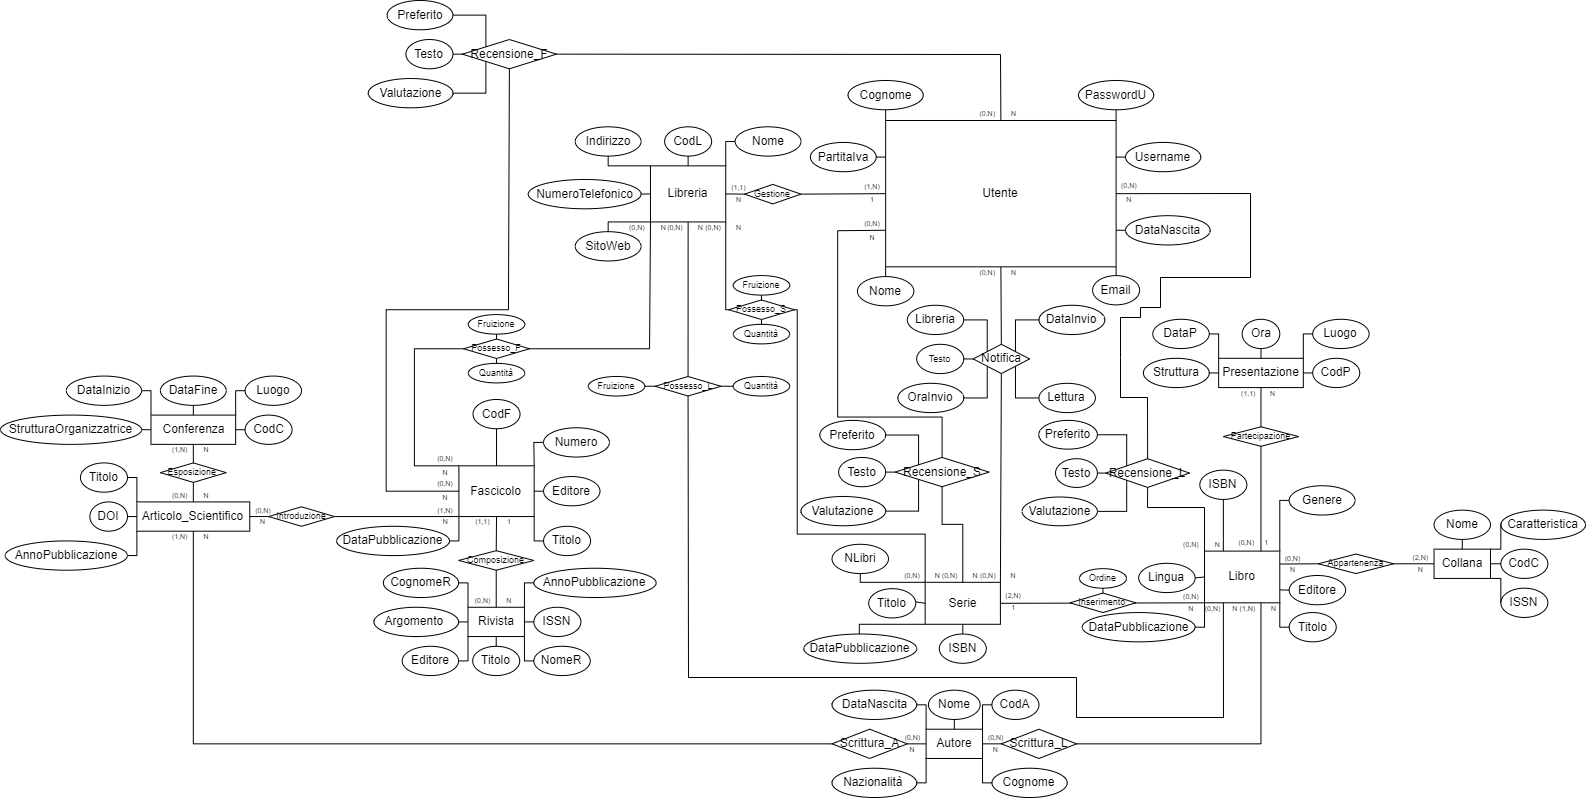
\includegraphics[width=0.75\columnwidth]{images/DiagrammaER v1.4.0(ristrutturato).png}
\end{figure}
\begin{figure}[htp!]
    \includegraphics[width=0.75\columnwidth]{images/DiagrammaUML(ristrutturato).png}
\end{figure}

\newpage
\section{Dizionari}

\subsection{Dizionario delle Entità}
\begin{table}[h]
\centering
\begin{tabular}{|p{5cm}|p{3cm}|p{7cm}|}
    \hline
    \textbf{Classi} & \textbf{Descrizione} & \textbf{Attributi} \\\hline

    UTENTE & Utente registrato al sistema. & \textbf{Username}(String): Indica l'username con il quale si identifica l'utente; \par
    \textbf{Email}(String): Indirizzo Email dell'utente; \par 
    \textbf{PasswordU}(String): Password d'accesso dell'utente; \par
    \textbf{PartitaIVA}(String): Partita IVA dell'utente che vuole registrare la propria libreria nel sistema; \par 
    \textbf{Nome}(String): Nome dell'utente; \par 
    \textbf{Cognome}(String): Cognome dell'utente.\\\hline

    LIBRERIA & Libreria gestista da un utente con la partita IVA. & \textbf{CodL}(Int): Codice che identifica la libreria; \par
    \textbf{NumeroTelefonico}(String): Numero di telefono della libreria; \par
    \textbf{SitoWeb}(String): Indirizzo Web della libreria; \par
    \textbf{Nome}(String): Nome della libreria; \par
    \textbf{Indirizzo}(String): Indirizzo della libreria; \par
    \textbf{Gestore}(String): Username dell'utente che gestisce la libreria.\\\hline
    
    RIVISTA & Rivista contenente i fascicoli. & \textbf{ISSN}(String): Identifica univocamente la rivista; \par
    \textbf{Argomento}(String): Argomento principale trattato nella rivista; \par
    \textbf{CognomeR}(String): Cognome del responsabile della rivista; \par
    \textbf{NomeR}(String): Nome del responsabile della rivista; \par
    \textbf{Titolo}(String): Titolo della rivista; \par
    \textbf{AnnoPubblicazione}(Int): Anno di pubblicazione della rivista.\\\hline
\end{tabular}
\end{table}

\newpage
\begin{table}[h]
\centering
\begin{tabular}{|p{5cm}|p{3cm}|p{7cm}|}
    \hline
    \textbf{Classi} & \textbf{Descrizione} & \textbf{Attributi} \\\hline  

    ARTICOLO\_SCIENTIFICO & Articolo scientifico (o pubblicazione) presente in un fascicolo di una rivista. & \textbf{DOI}(String): Identifica univocamente un articolo scientifico; \par
    \textbf{Titolo}(String): Titolo dell'artiolo scientifico; \par 
    \textbf{AnnoPubblicazione}(INT): Anno di pubblicazione dell'articolo scientifico.\\\hline

    FASCICOLO & Fascicolo di una rivista contenete degli articoli scientifici. & \textbf{CodF}(Int): Codice che identifica univocamente il fascicolo; \par
    \textbf{Numero}(Int): Numero del fascicolo in una rivista; \par
    \textbf{Editore}(String): Editore del fascicolo; \par
    \textbf{DataPubblicazione}(Date): Data di pubblicazione del fascicolo; \par
    \textbf{ISSN}(String): Rivista che contiene il fascicolo.\\\hline 

    CONFERENZA & Conferenza in cui sono stati pubblicati degli articoli scientifici. & \textbf{CodC}(Int): Codice che identifica univocamente la conferenza; \par
    \textbf{Luogo}(String): Indirizzo in cui è avvenuta la conferenza; \par
    \textbf{StrutturaOrganizzatrice}(String): Struttura che ha organizzato la conferenza; \par
    \textbf{DataInizio}(Date): Data in cui è iniziata la conferenza; \par
    \textbf{DataFine}(Date): Data in cui è finita la conferenza.\\\hline 

    SERIE & Serie di libri. & \textbf{ISBN}(String): Identifica univocamente la serie; \par
    \textbf{Titolo}(String): Titolo della serie; \par
    \textbf{DataPubblicazione}(Date): Data di pubblicazione della serie; \par
    \textbf{NLibri}(Int): Numero di libri che compongono la serie.\\\hline
\end{tabular}
\end{table}

\newpage
\begin{table}[h]
\centering
\begin{tabular}{|p{5cm}|p{3cm}|p{7cm}|}
    \hline
    \textbf{Classi} & \textbf{Descrizione} & \textbf{Attributi} \\\hline

    LIBRO & Libro registrato nel sistema. & \textbf{ISBN}(String): Identifica univocamente il libro; \par
    \textbf{Titolo}(String): Titolo del libro; \par 
    \textbf{Genere}(String): Genere del libro (didattico o romanzo); \par
    \textbf{Lingua}(String): Lingua in cui è scritto il libro; \par   
    \textbf{Editore}(String): Editore del libro; \par  
    \textbf{DataPubblicazione}(Date): Data di pubblicazione del libro.\\\hline

    PRESENTAZIONE & Presentazione in cui è stato esposto un libro. & \textbf{CodP}(Int):  Codice che identifica univocamente la presentazione; \par
    \textbf{Luogo}(String): Luogo in cui è avvenuta la presentazione; \par
    \textbf{Struttura}(String): Struttura in cui è stata organizzata la presentazione; \par
    \textbf{DataP}(Date): Data in cui è stata organizzata la presentazione; \par
    \textbf{ISBN}(String): Libro esposto durante la presentazione.\\\hline 

    COLLANA & Collana di libri che condividono una determinata caratteristica. & \textbf{CodC}(Int): Codice che identifica univocamente la collana; \par
    \textbf{Nome}(String): Nome della collana; \par
    \textbf{ISSN}(String): Identifica univocamente le collane che vengono pubblicate periodicamente; \par
    \textbf{Caratteristica}(String): Caratteristica condivisa dai libri della collana.\\\hline

    AUTORE & Autore di libri e/o articoli scientifici. & \textbf{CodA}(Int): Codice che identifica univocamente l'autore; \par 
    \textbf{Nome}(String): Nome dell'autore; \par
    \textbf{Cognome}(String): Cognome dell'autore; \par
    \textbf{Nazionalita}(String): Nazionalità dell'autore; \par
    \textbf{DataNascita}(Date): Data di nascita dell'autore.\\\hline
\end{tabular}
\end{table}

\newpage
\subsection{Dizionario delle Relazioni}
\begin{table}[h]
\centering
\begin{tabular}{|p{3cm}|p{5cm}|p{6cm}|}
    \hline
    \textbf{Relazioni} & \textbf{Descrizione} & \textbf{Attributi} \\\hline

    GESTIONE & Associazione: 'una-a-molti' che mette in relazione le librerie con l'utente che le gestisce. & \\\hline

    RECENSIONE\_F & Associazione: 'molti-a-molti' che mette in relazione i fascicoli con gli utenti che li hanno valutati, recensiti e/o inseriti nei preferiti. & \textbf{Username}(String): Username dell'utente che ha valutato, recensito e/o inserito il fascicolo nei preferiti; \par
    \textbf{CodF}(Int): Codice identificativo del fascicolo che è stato valutato, recensito, e/o inserito nei preferiti dall'utente; \par
    \textbf{Testo}(String): Testo di un'eventuale recensione scritta dall'utente; \par
    \textbf{Valutazione}(Int) Valore di un'eventuale valutazione fatta dall'utente; \par
    \textbf{Preferito}(Boolean): Indica se il fascicolo è stato inserito nei preferiti dall'utente.\\\hline

    RECENSIONE\_S & Associazione: 'molti-a-molti' che mette in relazione le serie di libri con gli utenti che li hanno valutate, recensite e/o inserite nei preferiti (attivando le notifiche). & \textbf{Username}(String): Username dell'utente che ha valutato, recensito e/o inserito la serie nei preferiti; \par
    \textbf{ISBN}(String) Serie che è stata valutata, recensita, e/o inserita nei preferiti dall'utente; \par
    \textbf{Testo}(String) Testo di un'eventuale recensione scritta dall'utente; \par
    \textbf{Valutazione}(Int) Valore di un'eventuale valutazione fatta dall'utente; \par
    \textbf{Preferito}(Boolean): Indica se l'utente ha inserito tra i preferiti la serie, e quindi vuole ricevere una notifia quando è disponibile presso una libreria.\\\hline 
\end{tabular}
\end{table}

\newpage
\begin{table}[h]
\centering
\begin{tabular}{|p{3cm}|p{5cm}|p{6cm}|}
    \hline
    \textbf{Relazioni} & \textbf{Descrizione} & \textbf{Attributi} \\\hline

    RECENSIONE\_L & Associazione: 'molti-a-molti' che mette in relazione i libri con gli utenti che li hanno valutati, recensiti e/o inseriti nei preferiti. & \textbf{Username}(String): Username dell'utente che ha valutato, recensito e/o inserito il libro nei preferiti; \par
    \textbf{ISBN}(String) Libro che è stato valutato, recensito, e/o inserito nei preferiti dall'utente; \par 
    \textbf{Testo}(String) Testo di un'eventuale recensione scritta dall'utente; \par
    \textbf{Valutazione}(Int) Valore di un'eventuale valutazione fatta dall'utente; \par
    \textbf{Preferito}(Boolean): Indica se il libro è stato inserito nei preferiti dall'utente.\\\hline

    POSSESSO\_F & Associazione: 'molti-a-molti' che mette in relazione i fascicoli con le librerie che li possiedono & \textbf{Fruizione}(String): Modalità di fruizione (Cartaceo, Digitale o AudioLibro) in cui è disponibile il fascicolo; \par
    \textbf{Quantità}(Int): Numero di fascicoli disponibili.\\\hline

    POSSESSO\_S & Associazione: 'molti-a-molti' che mette in relazione le serie con le librerie che le possiedono & \textbf{Fruizione}(String): Modalità di fruizione (Cartaceo, Digitale o AudioLibro) in cui è disponibile la serie; \par
    \textbf{Quantità}(Int): Numero di serie disponibili.\\\hline

    POSSESSO\_L & Associazione: 'molti-a-molti' che mette in relazione i libri con le librerie che li possiedono & \textbf{Fruizione}(String): Modalità di fruizione (Cartaceo, Digitale o AudioLibro) in cui è disponibile il fascicolo; \par
    \textbf{Quantità}(Int): Numero di libri disponibili.\\\hline
\end{tabular}
\end{table}

\newpage
\begin{table}[h]
\centering
\begin{tabular}{|p{3cm}|p{5cm}|p{6cm}|}
    \hline
    \textbf{Relazioni} & \textbf{Descrizione} & \textbf{Attributi} \\\hline

    NOTIFICA & Associazione: 'molti-a-molti' che contiene tutte le notifiche inviate & \textbf{Lettura}(Boolean): Indica se la notifica inviata è stata letta dall'utente che l'ha ricevuta; \par
    \textbf{Libreria}(Int): Codice identificativo della libreria che possiede tutta la serie; \par
    \textbf{Testo}(String): Testo della notifica inviata; \par
    \textbf{DataInvio}(Date): Data in cui è stata inviata la notifica, \par
    \textbf{OraInvio}(Orario): Ora in cui è stata inviata la notifica.\\\hline

    COMPOSIZIONE & Associazione: 'una-a-molti' che mette in relazione i fascicoli con la rivista che li contiene. &  \\\hline

    INTRODUZIONE & Associazione: 'molti-a-molti' che mette in relazione gli articoli scientifici con i fascicoli in cui sono introdotti. &  \\\hline

    ESPOSIZIONE & Associazione: 'molti-a-molti' che mette in relazione gli articoli scientifici con le conferenze in cui sono stati esposti. &  \\\hline

    INSERIMENTO & Associazione: 'una-a-molti' che mette in relazione i libri con la serie in cui sono stati inseriti. & \\\hline

    PARTECIPAZIONE & Associazione: 'una-a-molti' che mette in relazione le presentazioni con il libro che è stato presentato. &  \\\hline

    APPARTENENZA & Associazione: 'molti-a-molti' che mette in relazione i libri con le collane nelle quali sono stati inseriti. &  \\\hline
\end{tabular}
\end{table}

\newpage
\begin{table}[h]
\centering
\begin{tabular}{|p{3cm}|p{5cm}|p{6cm}|}
    \hline
    \textbf{Relazioni} & \textbf{Descrizione} & \textbf{Attributi} \\\hline
    
    SCRITTURA\_L & Associazione: 'molti-a-molti' che mette in relazione gli autori con i libri che hanno scritto. &  \\\hline

    SCRITTURA\_A & Associazione: 'molti-a-molti' che mette in relazione gli autori con gli articoli scientifici che hanno scritto. &  \\\hline
\end{tabular}
\end{table}  

\subsection{Dizionario dei Vincoli}
In questa sezione sono descritti tutti i vincoli necessari per garantire l'intregità semantica della base di dati.

\begin{itemize} 
    \item  \hypertarget{assertion1}{\textbf{ASSERTION A1}}: Garantisce che non esitano delle librerie con un gestore che non ha una partita IVA, evitando che vengano registrate delle librerie inesistenti.
        \begin{verbatim}
            CREATE ASSERTION A1
            CHECK(
                NOT EXISTS(
                    SELECT *
                    FROM UTENTE AS U JOIN LIBRERIA AS L ON U.Username=L.Gestore
                    WHERE U.PartitaIVA IS NULL
                )
            );
        \end{verbatim}
    Questo vincolo sarà imposto dai seguenti trigger:
        \begin{itemize}
            \item \hyperlink{t1}{T\_inserimentoLibreria}
            \item \hyperlink{t2}{T\_modificaGestore}
            \item \hyperlink{t3}{T\_modifca\_partitaIVA}
        \end{itemize}

    \item \hypertarget{assertion2}{\textbf{ASSERTION A2}}: Garantisce che non esistano degli articoli scientifici che sono stati pubblicati dopo i fascicoli in cui sono stati inseriti, evitando che vengano inseriti in dei fascicoli degli articoli scientifici quando quest ultimi non sono ancora stati pubblicati.
        \begin{verbatim}
            CREATE ASSERTION A2
            CHECK(
                NOT EXISTS(
                    SELECT *
                    FROM ((ARTICOLO_SCIENTIFICO AS AR JOIN INTRODUZIONE AS I ON
                        AR.DOI=I.DOI) JOIN FASCICOLO AS F ON F.CodF=I.CodF) 
                    WHERE AR.AnnoPubblicazione>EXTRACT(YEAR FROM F.DataPubblicazione)  
                )
            );
        \end{verbatim}
    Questo vincolo sarà imposto dai seguenti trigger:
        \begin{itemize}
            \item \hyperlink{t4}{T\_inserimentoIntroduzione}
            \item \hyperlink{t5}{T\_modificaIntroduzione}
            \item \hyperlink{t6}{T\_modificaFascicolo}
        \end{itemize}

    \item \hypertarget{assertion3}{\textbf{ASSERTION A3}}: Garantisce che non esitano dei fascicoli che sono stati pubblicati prima delle loro riviste, evitando che vengano inseriti dei fascicoli in delle riviste non ancora pubblicate.
        \begin{verbatim}
            CREATE ASSERTION A3
            CHECK(
                NOT EXISTS(
                    SELECT *
                    FROM FASCICOLO AS F JOIN RIVISTA AS R ON F.ISSN=R.ISSN
                    WHERE EXTRACT(YEAR FROM F.DataPubblicazione)<R.AnnoPubblicazione  
                )
            );
        \end{verbatim}
    Questo vincolo sarà imposto dai seguenti trigger:
        \begin{itemize}
            \item \hyperlink{t7}{T\_inserimentoFascicolo}
            \item \hyperlink{t6}{T\_modificaFascicolo}
            \item \hyperlink{t9}{T\_modificaRivista}
        \end{itemize}    

    \item \textbf{CONSTRAINT C1}: Garantisce che non vengano registrate confereze con la data di inzio succeessiva a quella di fine.
        \begin{verbatim}
            ALTER TABLE CONFERENZA
            ADD CONSTRAINT C1
            CHECK(
                DataInizio <= DataFine
            );
        \end{verbatim}
        
    \item \textbf{CONSTRAINT C2}: Viene utilizzato dal dominio 'isbn' garantendo che gli ISBN vengano scritti nel formato giusto.
        \begin{verbatim}
            CONSTRAINT C2
            CHECK (VALUE LIKE '978-%-%-_');
        \end{verbatim}
    
    \item \hypertarget{assertion4}{\textbf{ASSERTION A4}}: Garantisce che non esitano dei libri inseriti in una serie con l'ordine maggiore del numero di libri che contiene la serie in cui sono stati introdotti, evitando che vengano inseriti dei libri in una serie quando quest'ultima è stata già completata.
        \begin{verbatim}
            CREATE ASSERTION A4
            CHECK(
                NOT EXISTS(
                    SELECT *
                    FROM INSERIMENTO AS I JOIN SERIE AS S on I.Serie=S.isbn
                    WHERE S.NLibri<(
                    	                SELECT COUNT(Libro)
                                     FROM INSERIMENTO
                    	                WHERE Serie=S.isbn
                    )
                )
            );
        \end{verbatim}
    Questo vincolo sarà imposto dal seguente trigger:
        \begin{itemize}
            \item \hyperlink{t10}{T\_inserimentoLibroSerie}
        \end{itemize}
        
    \item \textbf{CONSTRAINT C3}: Viene utilizzato dal dominio 'fruizione' garantendo che la modalita di fruizione degli elementi venduti dalle librerie sia 'Cartaceo', 'Digitale' o 'AudioLibro'.
        \begin{verbatim}
            CONSTRAINT C3
            CHECK (VALUE IN ('Cartaceo', 'Digitale', 'AudioLibro'));
        \end{verbatim}

    \item \textbf{CONSTRAINT C4, C5 e C6}: Garantiscono che le quantità degli elementi disponibili (rispettivamente fascicoli, serie e libri) presso qualche libreria abbiano come valore NULL solo quando sono dipsonibili in formato Digitale o AudioLibro.
        \begin{verbatim}
            ALTER TABLE POSSESSO_F
            ADD CONSTRAINT C4
            CHECK((Quantita IS NOT NULL AND Fruizione='Cartaceo') OR (Quantita IS NULL 
                AND Fruizione IN ('AudioLibro', 'Digitale')));

            ALTER TABLE POSSESSO_S
            ADD CONSTRAINT C5
            CHECK((Quantita IS NOT NULL AND Fruizione='Cartaceo') OR (Quantita IS NULL 
                AND Fruizione IN ('AudioLibro', 'Digitale')));

            ALTER TABLE POSSESSO_L
            ADD CONSTRAINT C6
            CHECK((Quantita IS NOT NULL AND Fruizione='Cartaceo') OR (Quantita IS NULL 
                AND Fruizione IN ('AudioLibro', 'Digitale')));
        \end{verbatim} 

        \item \textbf{CONSTRAINT C7, C8 e C9}: Garantiscono che le valutazioni agli elementi che possono essere possededuti dalle librerie (rispettivamente fascicoli, serie e libri) abbiano un valore compreso in [1,5].
        \newpage
        \begin{verbatim}
            ALTER TABLE RECENSIONE_F
            ADD CONSTRAINT C7
            CHECK(Valutazione>=1 AND Valutazione<=5); 

            ALTER TABLE RECENSIONE_S
            ADD CONSTRAINT C8
            CHECK(Valutazione>=1 AND Valutazione<=5);

            ALTER TABLE RECENSIONE_L
            ADD CONSTRAINT C9
            CHECK(Valutazione>=1 AND Valutazione<=5);
        \end{verbatim} 

        \item \textbf{CONSTRAINT C10}: Viene utilizzato dal dominio 'issn' garantendo che gli ISSN vengano scritti nel formato giusto.
        \begin{verbatim}
            CONSTRAINT C10
            CHECK (VALUE LIKE '____-____');
        \end{verbatim}

        \item \textbf{CONSTRAINT C10}: Viene utilizzato dal dominio 'doi' garantendo che i DOI vengano scritti nel formato giusto.
        \begin{verbatim}
            CONSTRAINT C11
            CHECK (VALUE LIKE '10-%');
        \end{verbatim}

        \item \textbf{CONSTRAINT C12}: Garantisce che nella relazione 'RECENSIONE\_F' non ci siano dei fascicoli associati ad un utente che non l'ha valutato, recensito o inserito nei preferiti.
        \begin{verbatim}
            ALTER TABLE RECENSIONE_F
            ADD CONSTRAINT C12
            CHECK(NOT(Testo IS NULL AND Valutazione IS NULL AND Preferito=false));
        \end{verbatim}

        \item \textbf{CONSTRAINT C13}: Garantisce che nella relazione 'RECENSIONE\_S' non ci siano delle serie associate ad un utente che non l'ha valutata, recensita o inserita nei preferiti, e quindi non ha attivato le notifiche.
        \begin{verbatim}
            ALTER TABLE RECENSIONE_S
            ADD CONSTRAINT C13
            CHECK(NOT(Testo IS NULL AND Valutazione IS NULL AND Preferito=false));
        \end{verbatim}

        \item \textbf{CONSTRAINT C14}: Garantisce che nella relazione 'RECENSIONE\_L' non ci siano dei libri associati ad un utente che non l'ha valutato, recensito o inserito nei preferiti.
        \begin{verbatim}
            ALTER TABLE RECENSIONE_L
            ADD CONSTRAINT C14
            CHECK(NOT(Testo IS NULL AND Valutazione IS NULL AND Preferito=false));
        \end{verbatim}

        \item \textbf{CONSTRAINT C15}: Viene utilizzato dal dominio 'partitaiva' garantendo che le partite IVA dei gestori delle librerie vengano scritte nel formato giusto.
        \begin{verbatim}
            CONSTRAINT C15
            CHECK (VALUE LIKE '___________');
        \end{verbatim}

        \item \textbf{CONSTRAINT C16}: Garantisce che non vengano registrate delle librerie che non abbiano nè un sito web e nè un indirizzo.
        \begin{verbatim}
            ALTER TABLE LIBRERIA
            ADD CONSTRAINT C16
            CHECK(NOT(SitoWeb IS NULL AND Indirizzo IS NULL));
        \end{verbatim}

        \item \hypertarget{assertion5}{\textbf{ASSERTION A5}}: Garantisce che non esistano delle conferenze che iniziano prima della pubblicazione degli articoli scientifici esposti, evitando che vengano esposti in delle conferenze degli articoli che non sono ancora stati pubblicati.
        \begin{verbatim}
            CREATE ASSERTION A5
            CHECK(
                NOT EXISTS(
                    SELECT *
                    FROM ((CONFERENZA AS CO NATURAL JOIN ESPOSIZIONE AS E) 
                        NATURAL JOIN ARTICOLO_SCIENTIFICO AS AR) 
                    WHERE EXTRACT(YEAR FROM CO.DataInizio)<AR.AnnoPubblicazione
                )
            );
        \end{verbatim}
    Questo vincolo sarà imposto dai seguenti trigger:
        \begin{itemize}
            \item \hyperlink{t11}{T\_inserimentoEsposizione}
            \item \hyperlink{t12}{T\_modificaEsposizione}
            \item \hyperlink{t13}{T\_modifica\_pubblicazioneArticolo}
            \item \hyperlink{t14}{T\_modifica\_inizioConferenza}
        \end{itemize}   

    \item \hypertarget{assertion6}{\textbf{ASSERTION A6}}: Garantisce che non esistano delle presentazioni che iniziano prima della pubblicazione del libro presentato, evitando che vengano presentati dei libri che non sono ancora stati pubblicati.
        \begin{verbatim}
            CREATE ASSERTION A6
            CHECK(
                NOT EXISTS(
                    SELECT *
                    FROM LIBRO AS L NATURAL JOIN PRESENTAZIONE AS P  
                    WHERE P.DataP<L.DataPubblicazione
                )
            );          
        \end{verbatim}
    Questo vincolo sarà imposto dai seguenti trigger:
        \begin{itemize}
            \item \hyperlink{t15}{T\_inserimentoPresentazione}
            \item \hyperlink{t16}{T\_modificaPresentazione}
            \item \hyperlink{t17}{T\_modificaLibro}
        \end{itemize}
        
    \item \hypertarget{assertion7}{\textbf{ASSERTION A7}}: Garantisce che nell'associazione, che mette in relazione tutte le librerie con tutte le serie che possiedono, ovvero 'POSSESSO\_S', avviene un inserimento solo quando una libreria possiede tutti i libri che sono inseriti in una serie nella stessa modalità di fruizione. In oltre garantisce che la modalità di fruizione in 'POSSESSO\_S' sia la stessa di quella dei libri posseduti dalla libreria (cioè presenti in 'POSSESSO\_L') e che la quantità disponibile di una serie sia uguale al minor numero di libri della serie disponible nella libreria, solo quando la modalità di fruizione è cartacea.
    \newpage
        \begin{verbatim}
            SELECT COUNT(*)
            FROM ((((POSSESSO_S AS PS JOIN SERIE AS S ON PS.ISBN = S.ISBN) JOIN INSERIMENTO
                AS I ON S.ISBN = I.Serie) JOIN LIBRO AS L ON L.ISBN = I.Libro) 
                JOIN POSSESSO_L AS PL ON PL.ISBN=L.ISBN)
            WHERE PL.CodL = PS.CodL
            GROUP BY PL.CodL, PL.Fruizione, S.NLibri, PS.Fruizione, PS.Quantita, S.ISBN
            HAVING COUNT(*)<>S.NLibri OR (PS.Quantita <>(
                                                            SELECT MIN(Quantita)
                                                            FROM POSSESSO_L AS PL
                                                            WHERE PL.Fruizione='Cartaceo' AND 
                                                                ISBN IN(
                                                                        SELECT Libro
                                                                        FROM INSERIMENTO AS I
                                                                        WHERE I.Serie=S.ISBN
                                                                    )      
                                                        ) AND PS.Quantita IS NOT NULL)                    
        \end{verbatim}
    Questo vincolo sarà imposto dai seguenti trigger:
        \begin{itemize}
            \item \hyperlink{t18}{T\_inserimentoPossesso\_L}
            \item \hyperlink{t19}{T\_modificaPossesso\_L}
            \item \hyperlink{t20}{T\_eliminazionePossesso\_L}
        \end{itemize}  
\end{itemize}

\newpage
\section{Schema Logico e descrizioni}
\subsection{Schema Logico}
\begin{itemize} 
    \item \textbf{UTENTE}(\underline{Username}, Email, PasswordU, PartitaIVA, Nome, Cognome)
    \item \textbf{LIBRERIA}(\underline{CodL}, NumeroTelefonico, SitoWeb, Nome, Indirizzo, Gestore)
        \begin{itemize}
            \item LIBRERIA.Gestore → UTENTE.Username
        \end{itemize}
    \item \textbf{RIVISTA}(\underline{ISSN}, Editore, Argomento, CognomeR, NomeR, Titolo, AnnoPubblicazione)
    \item \textbf{ARTICOLO\_SCIENTIFICO}(\underline{DOI}, Titolo, AnnoPubblicazione)
    \item \textbf{FASCICOLO}(\underline{CodF}, Numero, Editore, Titolo, DataPubblicazione, ISSN)
        \begin{itemize}
	       \item FASCICOLO.ISSN→RIVISTA.ISSN
        \end{itemize}
    \item \textbf{INTRODUZIONE}(\underline{CodF, DOI})
        \begin{itemize}
	       \item INTRODUZIONE.CodF→FASCICOLO.CodF          
	       \item INTRODUZIONE.DOI→ARTICOLO\_SCIENTIFICO.DOI
        \end{itemize}
    \item \textbf{CONFERENZA}(\underline{CodC}, Luogo, StrutturaOrganizzatrice, DataInizio, DataFine)
    \item \textbf{ESPOSIZIONE}(\underline{DOI, CodC})
        \begin{itemize}
	       \item ESPOSIZIONE.DOI→ARTICOLO\_SCIENTIFICO.DOI
	       \item ESPOSIZIONE.CodC→CONFERENZA.CodC
        \end{itemize}
    \item \textbf{SERIE}(\underline{ISBN}, Titolo, ISSN, DataPubblicazione, NLibri)
    \item \textbf{LIBRO}(\underline{ISBN}, Titolo, Genere, Lingua, Editore,  DataPubblicazione)
    \item \textbf{INSERIMENTO}(\underline{Libro, Serie})
        \begin{itemize}
	       \item INSERIMENTO.Libro→LIBRO.ISBN
	       \item INSERIMENTO.Serie→SERIE.ISBN
        \end{itemize}
    \item \textbf{POSSESSO\_F}(\underline{CodL, CodF, Fruizione,} Quantità)
        \begin{itemize}    
            \item POSSESSO\_F.CodL→Libreria.CodL
            \item POSSESSO\_F.CodF→FASCICOLO.CodF
        \end{itemize}
    \item \textbf{RECENSIONE\_F}(\underline{Username, CodF,} Testo, Valutazione, Preferito)
        \begin{itemize}  
            \item RECENSIONE\_F.Username→UTENTE.Username
            \item RECENSIONE\_F.CodF→FASCICOLO.CodF
        \end{itemize}
    \item \textbf{POSSESSO\_S}(\underline{CodL, ISBN, Fruizione,} Quantità)
        \begin{itemize}
            \item POSSESSO\_S.CodL→Libreria.CodL
            \item POSSESSO\_S.ISBN→SERIE.ISBN
        \end{itemize}
    \item \textbf{RECENSIONE\_S}(\underline{Username, ISBN,} Testo, Valutazione, Preferito)
        \begin{itemize}
            \item PREFERITI\_S.Username→UTENTE.Username
            \item PREFERITI\_S.ISBN→SERIE.ISBN
        \end{itemize}
    \item \textbf{POSSESSO\_L}(\underline{CodL, ISBN, Fruizione,} Quantità)
        \begin{itemize}
            \item POSSESSO\_L.Username→UTENTE.Username
            \item POSSESSO\_L.CodL→LIBRERIA.CodL
        \end{itemize}
    \item \textbf{RECENSIONE\_L}(\underline{Username, ISBN,} Testo, Valutazione, Preferito)
        \begin{itemize} 
            \item PREFERITI\_L.Username→UTENTE.Username
            \item PREFERITI\_L.ISBN→LIBRO.ISBN
        \end{itemize}
    \item \textbf{NOTIFICA}(\underline{Username, ISBN, Libreria, OraInvio, DataInvio,} Lettura, Testo)
        \begin{itemize}        
            \item NOTIFICA.Username→UTENTE.Username
            \item NOTIFICA.ISBN→SERIE.ISBN
        \end{itemize}
    \item \textbf{PRESENTAZIONE}(\underline{CodP,} Luogo, Struttura, DataP, Ora, ISBN)
        \begin{itemize}        
            \item PRESENTAZIONE.ISBN→LIBRO.ISBN
        \end{itemize}
    \item \textbf{COLLANA}(\underline{CodC,} Nome, ISSN)
    \item \textbf{APPARTENENZA}(\underline{ISBN, CodC,} Caretteristica)
        \begin{itemize}        
            \item APPARTENENZA.ISBN→LIBRO.ISBN
            \item APPARTENENZA.CodC→COLLANA.CodC
        \end{itemize}
    \item \textbf{AUTORE}(\underline{CodA,} Nome, Cognome, Nazionalità, DataNascita)
    \item \textbf{SCRITTURA\_A}(\underline{DOI, CodA})
        \begin{itemize}        
            \item SCRITTURA\_A.DOI→ARTICOLO\_SCIENTIFICO.DOI
            \item SCRITTURA\_A.CodA→AUTORE.CodA
        \end{itemize}
    \item \textbf{SCRITTURA\_L}(\underline{ISBN, CodA})
        \begin{itemize}
            \item SCRITTURA\_L.ISBN→LIBRO.ISBN
            \item SCRITTURA\_L.CodA→AUTORE.CodA
        \end{itemize}
\end{itemize}

\subsection{Descrizione di Trigger}
Di seguito sono elencati tutti i Trigger utilizzati per la relizzazione della base di dati del sistema.
\begin{itemize}
    \item \hypertarget{t1}{\textbf{T\_inserimentoLibreria}}: il trigger si attiva dopo l'inserimento di una libreria e utilizza la funzione \hyperlink{f1}{'controllo\_inserimentoLibreria'} per garantire che i gestori delle librerie abbiano una Partita IVA, e quindi che il vincolo dell'assertion \hyperlink{assertion1}{A1} non sia violato.
    
    \item \hypertarget{t2}{\textbf{T\_modificaGestore}}: il trigger si attiva dopo un aggiornamento del campo 'Gestore' della tabella 'Libreria' e utilizza la funzione \hyperlink{f2}{'controllo\_modificaLibreria'} per garantire che il nuovo gestore della libreria abbia una Partita IVA, e quindi che il vincolo dell'assertion \hyperlink{assertion1}{A1} non sia violato. 

    \item \hypertarget{t3}{\textbf{T\_modifica\_partitaIVA}}: il trigger si attiva dopo un aggiornamenro del campo 'PartitaIVA' della tabella 'Utente' e utilizza la funzione \hyperlink{f3}{'controllo\_modifica\_PartitaIVA'} per garantire che la nuova Partita IVA non sia formata da dei caratteri che non sono numerici. In oltre, nel caso in cui la Partita IVA viene messa a "NULL", il trigger utilizza la funzione \hyperlink{f3}{'controllo\_modifica\_PartitaIVA'} anche per garantire che la libreria gestita dall'utente che ha chiuso la Partita IVA venga eliminata, e quindi che il vincolo dell'assertion \hyperlink{assertion1}{A1} non sia violato.

    \item \hypertarget{t4}{\textbf{T\_inserimentoIntroduzione}}: il trigger si attiva dopo un inserimento nella tabella 'Introduzione' e utilizza la funzione \hyperlink{f4}{'controllo\_introduzioneArticolo'} per garantire che in ogni fascicolo non ci siano degli articoli scientifici pubblicati dopo al fascicolo, e quindi che il vincolo dell'assertion \hyperlink{assertion2}{A2} non sia violato.

    \item \hypertarget{t5}{\textbf{T\_modificaIntroduzione}}: il trigger si attiva dopo un aggiornamento nella tabella 'Introduzione' e utilizza la funzione \hyperlink{f5}{'controllo\_modificaIntroduzione'} per garantire che nella tupla aggiornata non ci sia un articolo scientifico che è stato pubblicato dopo al fascicolo nel quale è stato introdotto, e quindi che il vincolo dell'assertion \hyperlink{assertion2}{A2} non sia violato.

    \item \hypertarget{t6}{\textbf{T\_modificaFascicolo}}: il trigger si attiva quando la data di pubblicazione di un fascicolo viene aggiornata con una data precedente a quella presente prima della modifica, oppure quando l'ISSN della rivista di un fascicolo viene modificato e utilizza la funzione \hyperlink{f6}{'controllo\_modificaFascicolo'} per garantire che la data di pubblicazione del fascicolo aggiornato non sia precedente a quella degli articoli contenuti nel fascicolo modificato e/o precedente alla rivista che contiene tale fascicolo, e quindi che i vincoli dell'assertion \hyperlink{assertion2}{A2} e \hyperlink{assertion2}{A3} non siano violati.

    \item \hypertarget{t7}{\textbf{T\_inserimentoFascicolo}}: il trigger si attiva dopo l'inserimento di un fascicolo e utilizza la funzione \hyperlink{f7}{'controllo\_inserimentoFascicolo'} per grantire che il fascicolo appena inserito faccia parte di una rivista pubblicata prima del fascicolo, e quindi che il vincolo dell'assertion \hyperlink{assertion3}{A3} non sia violato.

    \item \hypertarget{t9}{\textbf{T\_modificaRivista}}: il trigger si attiva quando l'anno di pubblicazione di una rivista viene aggiornata con una data più recente, oppure quando viene modificato l'ISSN di una rivista e utilizza la funzione \hyperlink{f9}{'controllo\_modificaRivista'} per garantire che la nuova data della rivista non sia successica a quella dei fascicoli che contiene, e quindi che il vincolo dell'asertion \hyperlink{assertion3}{A3} non sia violato.\\
     In oltre utilizza la funzione \hyperlink{f9}{'controllo\_modificaRivista'} anche per garantire che il nuovo ISSN non sia formato da dei caratteri che non sono numerici oppure il carattere '-'.

    \item \hypertarget{t10}{\textbf{T\_inserimentoLibroSerie}}: il trigger si attiva dopo un inserimento nella tabella 'Inserimento' e utilizza la funzione \hyperlink{f10}{'inserimento\_LibroSerie'} per garantire che in ogni serie non ci sia un numero di libri maggiore di quello indicato nel campo 'NLibri' della tabella 'Serie' e quindi che il vincolo dell'assertion \hyperlink{assertion4}{A4} non sia violato.

   \item \hypertarget{t11}{\textbf{T\_inserimentoEsposizione}}: il trigger si attiva dopo un inserimento nella tabella 'Esposizione' e utilizza la funzione \hyperlink{f11}{'controllo\_inserimentoEsposizione'} per garantire che nella tupla inserita non ci sia una conferenza di un articolo scientifico che è stato pubblicato dopo la data di inzio della conferenza, e quindi che il vincolo dell'asertion  \hyperlink{assertion5}{A5} non sia violato.

   \item \hypertarget{t12}{\textbf{T\_modificaEsposizione}}: il trigger si attiva dopo un aggiornamento nella tabella 'Esposizione' e utilizza la funzione \hyperlink{f12}{'controllo\_modificaEsposizione'} per garantire che nella tupla aggiornata non ci sia un articolo scientifico che è stato pubblicato dopo l'inizio della conferenza in cui è stato esposto, e quindi che il vincolo dell'assertion \hyperlink{assertion5}{A5} non sia violato.

   \item \hypertarget{t13}{\textbf{T\_modifica\_pubblicazioneArticolo}}: il trigger si attiva quando la data di pubbliazione di un articolo scientifico viene aggiornata con una data più recente e utilizza la funzione \hyperlink{f13}{'controllo\_modificaArticolo'} per garantire che la nuova data aggiornata non sia successiva a quella delle conferenze in cui è stato esposto l'articolo modificato, e quindi che il vincolo dell'assertion \hyperlink{assertion5}{A5} non sia violato.

   \item \hypertarget{t14}{\textbf{T\_modifica\_inizioConferenza}}: il trigger si attiva quando la data di inizio di una conferenza viene aggiornata con una data precedente a quella presente prima della modifica e utilizza la funzione \hyperlink{f14}{'controllo\_modificaConferenza'} per garantire che la nuova data di inizio non sia precedente a quella delle pubblicazioni degli articoli esposti nella conferenza modificata, e quindi che il vincolo dell'assertion \hyperlink{assertion5}{A5} non sia violato.

   \item \hypertarget{t15}{\textbf{T\_inserimentoPresentazione}}: il trigger si attiva dopo l'inserimento di una presentazione e utilizza la funzione \hyperlink{f15}{'controllo\_inserimentoPresentazione'} per garantire che alle presentazioni vengano esposti dei libri già pubblicati, e quindi che il vincolo dell'assertion \hyperlink{assertion6}{A6} non sia violato.

   \item \hypertarget{t16}{\textbf{T\_modificaPresentazione}}: il trigger si attiva dopo un aggiornamento del campo 'DataP' e/o 'ISBN' della tabella 'Presentazione' e quando la data viene aggiornata con un'altra che non è più recente di quella presente prima della modifica, il trigger utilizza la funzione \hyperlink{f16}{'controllo\_modificaPresentazione'} per garantire che la data della conferenza non sia precedente a quella della pubblicazione del libro presentato, e quindi che il vincolo dell'assertion \hyperlink{assertion6}{A6} non sia violato.

   \item \hypertarget{t17}{\textbf{T\_modificaLibro}}: il trigger si attiva quando la data di pubblicazione di un libro viene aggiornata con un'altra più recente, oppure quando viene modificato l'ISBN di un libro e utilizza la funzione \hyperlink{f17}{'controllo\_Libro'} per garantire che la nuova data non sia successiva a quelle delle presentazioni in cui è stato esposto il libro modificato, e quindi che il vincolo dell'assertion \hyperlink{assertion6}{A6} non sia violato.\\
   In oltre utilizza la funzione \hyperlink{f17}{'controllo\_Libro'} anche per garantire che il nuovo ISBN non sia formato da dei caratteri che non sono numerici oppure il carattere '-'.

   \item \hypertarget{t18}{\textbf{T\_inserimentoPossesso\_L}}: il trigger si attiva dopo un'inserimento nella tabella 'Possesso\_L', e quindi una libreria inizia a possedere un libro, il trigger utilizza la funzione \hyperlink{f18}{'controllo\_inserimentoPossesso\_L'} per far si che se il libro inserito appartiene a una serie e la libreria inserita nella nuova tupla inizia a possedere la serie di tale libro, allora avviene un inserimento nella tabella 'Possesso\_S' con la libreria, serie, modalità di fruizione e quantità giuste, e quindi garantisce che il vincolo dell'assertion \hyperlink{assertion7}{A7} non sia violato. 

   \item \hypertarget{t19}{\textbf{T\_modificaPossesso\_L}}: il trigger si attiva dopo l'aggiornamento del campo 'Quantita' della tabella 'Possesso\_L' e utilizza la funzione \hyperlink{f19}{'controllo\_modificaPossesso\_L'} per far si che se il libro modificato appartiene alla serie e la quantità aggiornata e la minore fra quelle dei libri della serie in cui è stato inserito il libro modificato, allora tale aggiornamento avviene anche nella tabella 'Possesso\_S', e quindi garantisce che il vincolo dell'assertion \hyperlink{assertion7}{A7} non sia violato.

   \item \hypertarget{t20}{\textbf{T\_eliminazionePossesso\_L}}: il trigger si attiva dopo un'eliminazione nella tabbella 'Possesso\_L', quindi una libreria non possiede più un libro, il trigger utilizza la funzione \hyperlink{f20}{'controllo\_eliminazionePossesso\_L'}, per far si che se il libro eliminato appartiene a una serie, allora viene eliminata anche la tupla nella tabella 'Possesso\_S' in cui sono in relazione la libreria e la serie del libro eliminato, e quindi garantisce che il vincolo dell'assertion \hyperlink{assertion7}{A7} non sia violato.

   \item \hypertarget{t21}{\textbf{T\_inserimentoArticolo}}: il trigger si attiva dopo l'inserimento di un articolo scientifico e utilizza la funzione \hyperlink{f21}{'inserimento\_DOIArticolo'} per garantire l'univocità dei DOI degli articoli scientifici.

   \item \hypertarget{t22}{\textbf{T\_inserimentoPossesso\_S}}: il trigger si attiva quando nella tabella 'Possesso\_S' viene inserta una tupla con il valore del campo 'Quantita' maggiore di 0, il trigger utilizza la funzione \hyperlink{f22}{'invia\_notifica\_possesso\_S'} per garantire che tutti gli utenti che hanno attivato le notifiche per la serie inserta, ricevano una notifica, e quindi avviene un inserimento nella tabella 'Notifica' con: gli utenti che hanno la serie inserita nei preferiti; la serie inserita e la libreria che la possiede.

   \item \hypertarget{t23}{\textbf{T\_modificaPossesso\_S}}: il trigger si attiva quando nella tabella 'Possesso\_S' viene aggiornato il valore del campo 'Quantita' da 0 a un valore maggiore di 0, il trigger utilizza la funzione \hyperlink{f22}{'invia\_notifica\_possesso\_S'} per garantire che tutti gli utenti che hanno attivato le notifiche per la serie nella tupla modificata, ricevano una notifica, e quindi avviene un inserimento nella tabella 'Notifica' con: gli utenti che hanno la serie inserita nei preferiti; la serie inserita e la libreria che la possiede.

   \item \hypertarget{t24}{\textbf{T\_inserimentoPreferiti\_S}}: il trigger si attiva quando viene inserita una tupla con il campo 'Preferito' a "true" nella tabella 'Recensione\_S', e quindi un utente ha attivato le notifiche per la serie inserita nella tupla, il trigger utilizza la funzione \hyperlink{f23}{'invia\_notifica\_preferiti\_S'} per garantire che l'utente he attivato le notifiche per una certa serie, riceva una notifica per ogni libreria che possiede la serie, e quindi per ognuna di queste librerie avviene un inserimento nella tabella 'Notifica' con: l'utente che ha attivato le notifiche; la serie inserita dall'utente nei preferiti e una libreria che la possiede.

   \item \hypertarget{t25}{\textbf{T\_modificaPreferiti\_S}}: il trigger si attiva quando viene aggiornato a "true" il valore del campo 'Preferito' nella tabella 'Recensione\_S', e quindi un utente ha attivato le notifiche per la serie inserita nella tupla modificata, il trigger utilizza la funzione \hyperlink{f23}{'invia\_notifica\_preferiti\_S'} per garantire che l'utente he attivato le notifiche per una certa serie, riceva una notifica per ogni libreria che possiede la serie, e quindi per ognuna di queste librerie avviene un inserimento nella tabella 'Notifica' con: l'utente che ha attivato le notifiche; la serie inserita dall'utente nei preferiti e una libreria che la possiede.

   \item \hypertarget{t26}{\textbf{T\_inserimentoRivista}}: il trigger si attiva dopo l'inserimento di una rivista e utilizza la funzione \hyperlink{f25}{controllo\_inserimentoRivista} per garantire che l'ISSN della nuova rivista non sia formato da dei caratteri che non sono numerici oppure il carattere '-'.

   \item \hypertarget{t27}{\textbf{T\_inserimentoCollana}}: il trigger si attiva dopo l'inserimento di una collana e utilizza la funzione \hyperlink{f26}{controllo\_inserimentoCollana} per garantire che un eventuale ISSN della nuova collana non sia formato da dei caratteri che non sono numerici oppure il carattere '-'.

   \item \hypertarget{t28}{\textbf{T\_modificaCollana}}: il trigger si attiva quando viene aggiornato l'ISSN di una collana con un valore diverso da "NULL" e utilizza la funzione \hyperlink{f27}{controllo\_modificaCollana} per garantire che il nuovo ISSN non sia formato da dei caratteri che non sono numerici oppure il carattere '-'.

   \item \hypertarget{t29}{\textbf{T\_inserimentoLibro}}: il trigger si attiva dopo l'inserimento di un libro e utilizza la funzione \hyperlink{f28}{controllo\_inserimentoLibro} per garantire che l'ISBN del nuovo libro non sia formato da dei caratteri che non sono numerici oppure il carattere '-'.

   \item \hypertarget{t30}{\textbf{T\_inserimentoSerie}}: il trigger si attiva dopo l'inserimento di una serie e utilizza la funzione \hyperlink{f29}{controllo\_inserimentoSerie} per garantire che l'ISBN della nuova serie non sia formato da dei caratteri che non sono numerici oppure il carattere '-'.

   \item \hypertarget{t31}{\textbf{T\_modificaSerie}}: il trigger si attiva dopo l'aggiornamento dell'ISBN di una serie e utilizza la funzione \hyperlink{f30}{controllo\_modificaSerie} per garantire che il nuovo ISBN non sia formato da dei caratteri che non sono numerici oppure il carattere '-'.

    \item \hypertarget{t32}{\textbf{T\_inserimentoUtente}}: il trigger si attiva quando viene inserito un utente con una Partita IVA diversa da "NULL" e utilizza la funzione \hyperlink{f31}{controllo\_inserimentoUtente} per garantire che un'eventuale Partita IVA del nuovo utente non sia formato da dei caratteri che non sono numerici.
    
\end{itemize}

\subsection{Descrizioni di Funzioni e Procedure}
Di seguito sono elencati tutte le funzioni e le procedure utilizzate per la relizzazione della base di dati del sistema.

\begin{itemize}
    \item \hypertarget{f1}{\textbf{controllo\_inserimentoLibreria}}:\\
    la funzione viene richiamata dal trigger \hyperlink{t1}{'T\_inserimentoLibreria'} e se viene inserita una nuova libreria con un gestore che non ha una Partita IVA, allora la funzione elimina questa libreria.

    \item \hypertarget{f2}{\textbf{controllo\_modificaLibreria}}:\\
    la funzione viene richiamata dal trigger \hyperlink{t2}{'T\_modificaGestore'} e se viene aggiornato il gestore di una libreria con un altro che non possiede una Partita IVA, allora la funzione annulla l'aggiornamento, inserendo di nuovo il vecchio gestore nella tupla modificata.

    \item \hypertarget{f3}{\textbf{controllo\_modifica\_PartitaIVA}}:\\
    la funzione viene richiamata dal trigger \hyperlink{t3}{'T\_modifica\_partitaIVA'} e se il nuovo valore della Partita IVA non è "NULL", e se la nuova Partita IVA ha un carattere che non è numerico, allora annulla l'aggiornamento, inserendo di nuovo il vecchio valore dell'ISBN nella tupla modificata, altrimenti, se il nuovo valore è "NULL", allora la funzione elimina tutte le librerie dell'utente che ha chiuso la partita IVA.

    \item \hypertarget{f4}{\textbf{controllo\_introduzioneArticolo}}:\\
    la funzione viene richiamata dal trigger \hyperlink{t4}{'T\_inserimentoIntroduzione'} e se viene inserita nella tabella 'Introduzione' una tupla in cui l'anno di pubblicazione dell'articolo scientifico è più recente di quello del fascicolo, allora la funzione elimina questa tupla.

    \item \hypertarget{f5}{\textbf{controllo\_modificaIntroduzione}}:\\
    la funzione viene richiamata dal trigger \hyperlink{t5}{'T\_modificaIntroduzione'} e se viene aggiornata nella tabella 'Introduzione' una tupla in cui l'anno di pubblicazione dell'articolo scientifico è piu recente di quello del fascicolo, allora la funzione annulla la modifica, riportando i valori dei campi della tupla aggiornata a quelli precedenti alla modifica.

    \item \hypertarget{f6}{\textbf{controllo\_modificaFascicolo}}:\\
    la funzione viene richiamata dal trigger \hyperlink{t6}{'T\_modifica\_pubblicazioneFascicolo'} quando la data di pubblicazione di un fascicolo viene aggiornata con un'altra precedente a quella presente prima della modifica, oppure quando viene modificato l'ISSN della rivista di un fascicolo, quindi se il nuovo anno di pubblicazione del fascicolo aggiornato è precedente a quello di un articolo inserito in tale fascicolo, oppure è precedente a quello della nuova rivista, allora la funzione annulla l'aggiornamento, inserendo di nuovo la vecchia data di pubblicazione e/o il vecchio ISSN nella tupla aggiornata.

    \item \hypertarget{f7}{\textbf{controllo\_inserimentoFascicolo}}:\\
    la funzione viene richiamata dal trigger \hyperlink{t7}{'T\_inserimentoFascicolo'} e se viene inserito un nuovo fascicolo con una data pubblicazione di cui l'anno è precedente a quello della sua rivista, allora la funzione elimina questo fascicolo.

    \item \hypertarget{f9}{\textbf{controllo\_modificaRivista}}:\\
    la funzione viene richiamata dal trigger \hyperlink{t9}{'T\_modificaRivista'} quando l'anno di pubblicazione di una rivista viene aggiornato con un'altro più recente, oppure quando viene modificato l'ISSN di una rivista, quindi se il nuovo anno di pubblicazione è più recente di quello di qualche fascicolo contenuto dalla rivista modificata, allora la funzione annulla l'aggiornamento, riportando il valore dell'anno di pubblicazione della rivista a quello precedente alla modifica.\\
    In oltre utilizza la funzione \hyperlink{f24}{'controlla\_formato'} per controllare se il nuovo ISSN della rivista appena modificata ha un carattere che non è numerico oppure il carattere '-', in tal caso annulla l'aggiornamento, inserendo di nuovo il vecchio valore dell'ISSN nella tupla modificata. 

    \item \hypertarget{f10}{\textbf{inserimento\_LibroSerie}}:\\
    la funzione viene richiamata dal trigger \hyperlink{t10}{'T\_inserimentoLibroSerie'} e se nella tabella 'Inserimento' sono stati inseriti tutti i libri della serie (e quindi la serie è già stata completata), allora la funzione elimina la tupla inserita.

    \item \hypertarget{f11}{\textbf{controllo\_inserimentoEsposizione}}:\\
    la funzione viene richiamata dal trigger \hyperlink{t11}{'T\_inserimentoEsposizione'} e se viene inserita una tupla nella tabella 'Esposizione' in cui l'articolo scientifico ha un anno di pubblicazione successivo a quello dell'inizio della conferenza, allora la funzione elimina questa tupla.

    \item \hypertarget{f12}{\textbf{controllo\_modificaEsposizione}}:\\
    la funzione viene richiamata dal trigger \hyperlink{t12}{'T\_modificaEsposizione'} e se viene aggiornata una tupla nella tabella 'Esposizione' in cui l'anno di pubblicazione dell'articolo scietifico è più recente di quello di inizio della conferenza, allora la funzione annula la modifica, riportando i valori dei campi della tupla aggiornata a quelli precedenti alla modifica. 

    \item \hypertarget{f13}{\textbf{controllo\_modificaArticolo}}:\\
    la funzione viene richiamata dal trigger \hyperlink{t13}{'T\_modifica\_pubblicazioneArticolo'} quando l'anno di pubblicazione di un articolo scientifico viene aggiornato con un'altro più recente, quindi se il nuovo anno di pubblicazione è più recente di quello di inizio di qualche conferenza in cui è stato esposto, allora la funzione annulla la modifica, riportando il valore dell'anno di pubblicazione dell'articolo a quello precedente all'aggiornamento.

    \item \hypertarget{f14}{\textbf{controllo\_modificaConferenza}}:\\
    la funzione viene richiamata dal trigger \hyperlink{t14}{'T\_modifica\_inizioConferenza'} quando la data di inizio di una conferenza viene aggiornata con una data precedente a quella presente prima della modifica, quindi se l'anno della nuova data di inzio della conferenza è precedete a quello di qualche articolo esposto nella conferenza modificata, allora la funzione annulla l'aggiornamento, inserendo di nuovo la vecchia data di inzio della conferenza nella tupla modificata.

    \item \hypertarget{f15}{\textbf{controllo\_inserimentoPresentazione}}:\\
    la funzione viene richiamata dal trigger \hyperlink{t15}{'T\_inserimentoPresentazione'} e se viene inserita una presentazione con una data precedente a quella della pubblicazione del libro, allora la funzione elimina questa presentazione.

    \item \hypertarget{f16}{\textbf{controllo\_modificaPresentazione}}:\\
    la funzione viene richiamata dal trigger \hyperlink{t16}{'T\_modificaPresentazione'} quando l'ISBN del libro di una presentazione viene aggiornato oppure la data della presentazione viene aggiornata con un'altra più vecchia, quindi se nella tupla modificata la data della presentazione è precedente a quella della pubblicazione del libro, allora la funzione annulla l'aggiornamento riportando i valori dei campi 'DataP' e 'ISBN' della tabella 'Presentazione' ai valori precedenti alla modifica della tupla.

    \item \hypertarget{f17}{\textbf{controllo\_Libro}}:\\
    la funzione viene richiamata dal trigger \hyperlink{t17}{'T\_modificaLibro'} quando la data di pubblicazione di un libro viene aggiornata con un'altra più recente, quindi se la nuova data è successiva a quella di qualche presentazione del libro, allora la funzione annulla la modifica, inserendo di nuovo la vecchia data nella tupla aggiornata.\\
    In oltre utilizza la funzione \hyperlink{f24}{'controlla\_formato'} per controllare se il nuovo ISBN del libro appena modificato ha un carattere che non è numerico oppure il carattere '-', in tal caso annulla l'aggiornamento, inserendo di nuovo il vecchio valore dell'ISBN nella tupla modificata. 

    \item \hypertarget{f18}{\textbf{controllo\_inserimentoPossesso\_L}}:\\
    la funzione viene richiamata dal trigger \hyperlink{t18}{'T\_inserimentoPossesso\_L'} e se dopo l'inserimento di una tupla nella tabella 'Possesso\_L' una libreria inizia a possedere tutti i libri di una serie nello stesso formato, allora la funzione effettua un inserimento nella tabella 'Possesso\_S' con: 
    \begin{itemize}
        \item il codice della libreria che possiede la serie completa;
        \item l'ISBN della serie;
        \item la modalità di fruizione del libro inserito nella nuova tupla di 'Possesso\_L';
        \item e la quantità disponibile con un valore pari a quello minore delle disponibilità dei libri della serie inserita solo quando la modalità di fruizione è 'Cartaceo'.
    \end{itemize}    

    \item \hypertarget{f19}{\textbf{controllo\_modificaPossesso\_L}}:\\
    la funzione viene richiamata dal trigger \hyperlink{t19}{'T\_modificaPossesso\_L'} quando la quantità disponibile di un libro presso una libreria viene modificata, e se questo libro appartiene a una serie disponibile presso la stessa libreria, allora la funzione aggiorna la quantità disponibile di tale serie in questa libreria con il numero minore di disponibilità dei libri della serie posseduti dalla libreria.

    \item \hypertarget{f20}{\textbf{controllo\_eliminazionePossesso\_L}}:\\
    la funzione viene richiamata dal trigger \hyperlink{t20}{'T\_eliminazionePossesso\_L'} e se dopo un'eliminazione di una tupla nella tabella 'Possesso\_L' una libreria non possiede più tutti i libri di una serie, allora la funzione elimina la tupla della tabella 'Possesso\_S' con:
    \begin{itemize}
        \item l'ISBN della serie; 
        \item il codice della libreria che non possiede più il libro; 
        \item la modalità di fruizione del libro eliminato;
    \end{itemize} 

    \item \hypertarget{f21}{\textbf{inserimento\_DOIArticolo}}:\\
    la funzione viene richiamata dal trigger \hyperlink{t21}{'T\_inserimentoArticolo'} e completa l'inserimento di un articolo scientifico aggiungendo il DOI che identifica univocamente l'articolo appena inserito.

    \item \hypertarget{p1}{\textbf{invia\_notifica}}:\\
    la procedura riceve come parametri di input l'username di un untente; l'ISBN di una serie; il codice di una libreria e una modalità di fruizione. La procedura utilizza questi parametri per inviare una notifica all'utente con l'username ricevuto, cioè inserisce nella tabella 'Notifica' una tupla con: l'username dell'utente; l'ISBN della serie; il codice della libreria che possiede la serie; la data e l'ora di invio della notifica e un testo con tutte le informazioni della libreria e della serie disponibile. 

    \item \hypertarget{f22}{\textbf{invia\_notifica\_possesso\_S}}:\\
    la funzione viene richiamata dal trigger \hyperlink{t22}{'T\_inserimentoPossesso\_S'}, quando la quantità disponibile della serie inserita è maggiore di 0, e dal trigger \hyperlink{t23}{'T\_modificaPossesso\_S'}, quando la quantità disponibile della serie viene aggiornata da 0 a un valore maggiore di 0, quindi la funzione invia a tutti gli utenti, che hanno attivato le notifiche per la serie inserita o aggiornata, una notifica utilizzando la procedura  \hyperlink{p1}{'invia\_notifica'}.

    \item \hypertarget{f23}{\textbf{invia\_notifica\_preferiti\_S}}:\\
    la funzione viene richiamata dai trigger \hyperlink{t24}{'T\_inserimentoPreferiti\_S'} e \hyperlink{t25}{'T\_modificaPreferiti\_S'} quando nella tabella 'Recensione\_S' viene inserita o aggiornata una tupla con il campo 'Preferito' a "true", quindi la funzione invia all'utente, che ha inserito una serie nei preferiti, una notifica per ogni libreria che possiede tale serie utilizzando la procedura \hyperlink{p1}{'invia\_notifica'}.

    \item \hypertarget{f24}{\textbf{controlla\_formato}}:\\
    la funzione riceve come parametri di input una stringa e manda come parametro di output "false" se tale stringa contiene dei caratteri che non sono nè dei numeri e nè il carattere '-'.

    \item \hypertarget{f25}{\textbf{controllo\_inserimentoRivista}}:\\
    la funzione viene richiamata dal trigger \hyperlink{t26}{'T\_inserimentoRivista'} e utilizza la funzione \hyperlink{f24}{'controlla\_formato'} per controllare se l'ISSN della rivista appena inserita ha un carattere che non è numerico oppure il carattere '-', in tal caso annulla l'inserimento, eliminando la tupla appena inserita.

    \item \hypertarget{f26}{\textbf{controllo\_inserimentoCollana}}:\\
    la funzione viene richiamata dal trigger \hyperlink{t27}{'T\_inserimentoCollana'} e utilizza la funzione \hyperlink{f24}{'controlla\_formato'} per controllare se un eventuale ISSN della collana appena inserita ha un carattere che non è numerico oppure il carattere '-', in tal caso annulla l'inserimento, eliminando la tupla appena inserita.

    \item \hypertarget{f27}{\textbf{controllo\_modificaCollana}}:\\
    la funzione viene richiamata dal trigger \hyperlink{t28}{'T\_inserimentoCollana'} e utilizza la funzione \hyperlink{f24}{'controlla\_formato'} per controllare se il nuovo ISSN della collana appena modificata ha un carattere che non è numerico oppure il carattere '-', in tal caso annulla l'aggiornamento, inserendo di nuovo il vecchio valore dell'ISSN nella tupla appena modificata. 

    \item \hypertarget{f28}{\textbf{controllo\_inserimentoLibro}}:\\
    la funzione viene richiamata dal trigger \hyperlink{t29}{'T\_inserimentoLibro'} e utilizza la funzione \hyperlink{f24}{'controlla\_formato'} per controllare se l'ISBN del libro appena inserito ha un carattere che non è numerico oppure il carattere '-', in tal caso annulla l'inserimento, eliminando la tupla appena inserita.

    \item \hypertarget{f29}{\textbf{controllo\_inserimentoSerie}}:\\
    la funzione viene richiamata dal trigger \hyperlink{t30}{'T\_inserimentoSerie'} e utilizza la funzione \hyperlink{f24}{'controlla\_formato'} per controllare se l'ISBN della serie appena inserita ha un carattere che non è numerico oppure il carattere '-', in tal caso annulla l'inserimento, eliminando la tupla appena inserita.

    \item \hypertarget{f30}{\textbf{controllo\_modificaSerie}}:\\
    la funzione viene richiamata dal trigger \hyperlink{t31}{'T\_modificaSerie'} e utilizza la funzione \hyperlink{f24}{'controlla\_formato'} per controllare se il nuovo ISBN della serie appena modificata ha un carattere che non è numerico oppure il carattere '-', in tal caso annulla l'aggiornamento, inserendo di nuovo il vecchio valore dell'ISBN nella tupla appena modificata.

    \item \hypertarget{f31}{\textbf{controllo\_inserimentoUtente}}:\\
    la funzione viene richiamata dal trigger \hyperlink{t32}{'T\_inserimentoUtente'} e utilizza la funzione \hyperlink{f24}{'controlla\_formato'} per controllare se un'eventuale Partita IVA del utente appena inserito ha un carattere che non è numerico, in tal caso annulla l'inserimento, eliminando la tupla appena inserita.
\end{itemize}

\end{document}
